% Section 5: Results
% NOTE: \section{Results} and \label{sec:results} are in main.tex

We evaluate \epikg through two benchmarks: ClinicalBench tests assertion-sensitive and longitudinal reasoning, while SliceBench measures longitudinal QA across patient complexity tiers.
ClinicalBench uses a deterministic keyword evaluator for reproducibility; SliceBench uses LLM-as-judge evaluation (Section~\ref{sec:bench:protocol}).
Claude Opus 4.6 is the primary answering model; MedGemma 27B and GPT-OSS 20B provide cross-model validation.
Both benchmarks report bias-corrected and accelerated (BCa) bootstrap 95\% CIs ($n=2{,}000$, seed 42)~\cite{efron1993bootstrap}, resampled at the question level.

% ----------------------------------------------------------
\subsection{ClinicalBench: Primary Ablation}
\label{sec:results:clinicalbench}

\begin{table}[t]
\centering
\caption{ClinicalBench primary results (400 questions, Claude Opus 4.6, keyword evaluator v2 with abstention detection). C7 is model-independent (no LLM); remaining conditions use Opus 4.6. Sig: * denotes BCa CI excluding zero. Best in \textbf{bold}.}
\label{tab:clinicalbench_ablation}
\small
\begin{tabular}{@{}llcl@{}}
\toprule
& Condition & Accuracy & $\Delta$ vs C1 \\
\midrule
C7 & Deterministic KG (no LLM) & 3.8\% & $-18.7\pp$ \\
\midrule
C1 & LLM Alone & 22.5\% & --- \\
C4g & + Intent-Aware KG-RAG & \textbf{69.0\%} & $+46.5\pp$ * \\
\midrule
C6 & Long Context (all notes) & 40.2\% & $+17.8\pp$ \\
\bottomrule
\end{tabular}
\end{table}

The bookend baselines bracket the design space: C7 (deterministic KG, no LLM) achieves 3.8\%---only negation detection works (13.6\%) via stored assertion metadata---confirming that an LLM is essential for reasoning over graph evidence.
C6 (all notes concatenated) scores 40.2\%, outperforming C1 ($+17.8\pp$) because it at least provides clinical text for the model to reason over, but it still falls far short of C4g and catastrophically fails on historical (0\%) and sequence (0\%).
Intent-aware KG-RAG (C4g) reaches 69.0\% ($+46.5\pp$ vs.\ C1; 95\% BCa CI: \ci{+40.2\pp}{+52.0\pp}), confirming that question-type-specific graph traversal is critical.
Without retrieval, the model mostly abstains or produces vague responses that fail keyword matching; with structured retrieval, it produces substantive correct answers.

% ----------------------------------------------------------
\subsection{Category$\times$Condition Interaction}
\label{sec:results:categories}

\begin{table}[t]
\centering
\caption{ClinicalBench per-category accuracy (\%) across conditions (Claude Opus 4.6, evaluator v2). C4g improves all 9 categories over C1. Best per row in \textbf{bold}.}
\label{tab:clinicalbench_categories}
\small
\begin{tabular}{@{}lccccl@{}}
\toprule
Category & $n$ & C6 & C1 & C4g & C4g$-$C1 \\
\midrule
Negation & 110 & 69.1 & 45.5 & \textbf{80.9} & $\uparrow 35.5\pp$ \\
Conditional & 20 & 35.0 & 0.0 & \textbf{45.0} & $\uparrow 45.0\pp$ \\
Uncertainty & 40 & 27.5 & 12.5 & \textbf{50.0} & $\uparrow 37.5\pp$ \\
Family hist. & 30 & 43.3 & 3.3 & \textbf{56.7} & $\uparrow 53.3\pp$ \\
Sequence & 40 & 0.0 & 10.0 & \textbf{65.0} & $\uparrow 55.0\pp$ \\
\midrule
Current st. & 50 & 44.0 & 26.0 & \textbf{70.0} & $\uparrow 44.0\pp$ \\
Duration & 30 & 66.7 & 30.0 & \textbf{66.7} & $\uparrow 36.7\pp$ \\
Historical & 50 & 0.0 & 6.0 & \textbf{60.0} & $\uparrow 54.0\pp$ \\
Change & 30 & 40.0 & 16.7 & \textbf{100.0} & $\uparrow 83.3\pp$ \\
\midrule
\textbf{Overall} & \textbf{400} & 40.2 & 22.5 & \textbf{69.0} & $\uparrow 46.5\pp$ \\
\bottomrule
\end{tabular}
\end{table}

\begin{figure}[t]
\centering
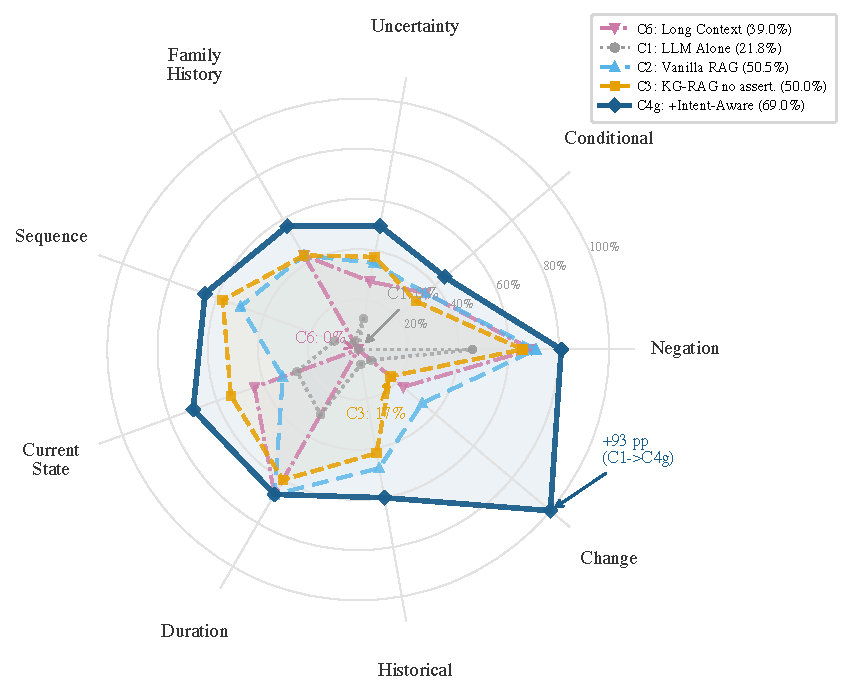
\includegraphics[width=\textwidth]{figures/fig2_radar.pdf}
\caption{ClinicalBench per-category accuracy across three conditions (C6, C1, C4g; Claude Opus 4.6, evaluator v2). C6 (pink dash-dot) collapses on historical and sequence (both 0\%); C1 (gray dotted) falls below 50\% on 7 of 9 categories, reflecting frequent abstentions without retrieval context; C4g (dark solid) improves all 9 categories over C1.}
\label{fig:radar}
\end{figure}

Table~\ref{tab:clinicalbench_categories} and Figure~\ref{fig:radar} reveal a strong \emph{category$\times$condition interaction}: intent-aware KG-RAG improves all 9 categories over C1, with every delta exceeding $+35\pp$.
Under the v2 evaluator with abstention detection, C1 drops sharply because the model without retrieval context frequently abstains (``insufficient information in the notes'') rather than attempting an answer.

\paragraph{Where intent-aware routing excels.}
\begin{sloppypar}
The largest gains occur on categories requiring cross-admission synthesis: change ($+83\pp$), sequence ($+55\pp$), historical ($+54\pp$), family history ($+53\pp$), conditional ($+45\pp$), and current state ($+44\pp$).
On the hard longitudinal subset (change + current state + historical, $n=130$), C4g outperforms C1 by $+56.9\pp$ (95\% BCa CI: \ci{+46.2\pp}{+65.4\pp}).
All nine category improvements exceed $+35\pp$ (Appendix Figure~\ref{fig:deltas}).
C6 fails catastrophically on historical (0\%) and sequence (0\%) despite Opus's 200K window, confirming that long context cannot substitute for structured retrieval on these categories.
\end{sloppypar}

% ----------------------------------------------------------
\subsection{Cross-Model Validation}
\label{sec:results:crossmodel}

\begin{table}[t]
\centering
\caption{ClinicalBench cross-model results (400 questions, keyword evaluator v2). All three models benefit from KG-RAG; the largest gain accrues to the most capable general-purpose model.}
\label{tab:crossmodel}
\small
\begin{tabular}{@{}llccl@{}}
\toprule
& Model & C1 & C4g & $\Delta$ \\
\midrule
Commercial & Claude Opus 4.6 & 22.5\% & \textbf{69.0\%} & $+46.5\pp$ \\
Open & GPT-OSS 20B & 20.8\% & 59.2\% & $+38.5\pp$ \\
Medical & MedGemma 27B & 26.5\% & 58.1\% & $+31.6\pp$ \\
\bottomrule
\end{tabular}
\end{table}

All three models benefit substantially from KG-RAG (Table~\ref{tab:crossmodel}), with the magnitude inversely related to parametric medical knowledge.
Opus gains $+46.5\pp$, GPT-OSS gains $+38.5\pp$, and MedGemma---the only model fine-tuned on medical corpora---gains $+31.6\pp$.
Notably, MedGemma starts with the highest C1 baseline (26.5\%) yet achieves the lowest C4g accuracy (58.1\%), while Opus starts at 22.5\% but reaches 69.0\% with retrieval.

All three models improve on all 9 categories under C4g (per-category cross-model breakdowns in Appendix Table~\ref{tab:crossmodel_categories}).
Intent-aware KG-RAG thus functions as a \emph{medical knowledge compensator}: the structured epistemic context partially substitutes for parametric medical knowledge, providing the largest benefit to general-purpose models that need it most.

% ----------------------------------------------------------
\subsection{SliceBench}
\label{sec:results:slicebench}

\begin{table}[t]
\centering
\caption{SliceBench overall results (144 questions, Claude Sonnet 4.5, judged by Opus 4.6). Sig: * denotes CI excluding zero.}
\label{tab:slicebench_overall}
\small
\begin{tabular}{@{}llccc@{}}
\toprule
& Condition & Score & 95\% CI & $\Delta$ vs B0 \\
\midrule
B0 & LLM Alone & 49.9\% & \ci{43.6\%}{56.1\%} & --- \\
B1 & Latest Note & 73.4\% & \ci{67.8\%}{78.7\%} & $+23.5\pp$ \\
B2 & All Notes RAG & 84.7\% & \ci{80.2\%}{88.8\%} & $+34.8\pp$ * \\
B3 & KG-RAG & 86.9\% & \ci{82.8\%}{90.8\%} & $+37.0\pp$ * \\
B4 & Full System & 87.6\% & \ci{83.7\%}{91.2\%} & $+37.8\pp$ * \\
\bottomrule
\end{tabular}
\end{table}

The incremental KG layer (B2$\rightarrow$B3) contributes $+2.2\pp$ overall (CI: \ci{-1.5\pp}{+5.9\pp}), not reaching aggregate significance, but tier-stratified estimates show a complexity-dependent trend: $+0.6\pp$ (Tier~A), $+1.0\pp$ (Tier~B), $+5.0\pp$ (Tier~C, 15+ encounters), consistent with KG context being most valuable when document volume overwhelms chunk-level retrieval (Appendix~\ref{app:slicebench_tiers}).

% ----------------------------------------------------------
\subsection{Physician Adjudication}
\label{sec:results:physician}

A two-physician blinded adjudication ($n=168$ questions $\times$ 2 conditions, Cohen's $\kappa$ for inter-rater reliability) is preregistered to validate automated scoring; the protocol (Appendix~\ref{app:physician_protocol}) was designed before examining results. \emph{Results are pending.}
